\chapter{Introduction}
% ------------------------

\section{Aim and Background}
The aim of this project was to design an automated chip tester for the University
of Southampton Superchip, also known as D2. Undergraduates at the School of Electronics
and Computer Science participate every year in a project in which they
design a part of a digital chip. Figure \ref{fig:chip_overview} shows an overview
of the final chip, which includes up to 16 individual designs.
\begin{figure}[h!]
\centering
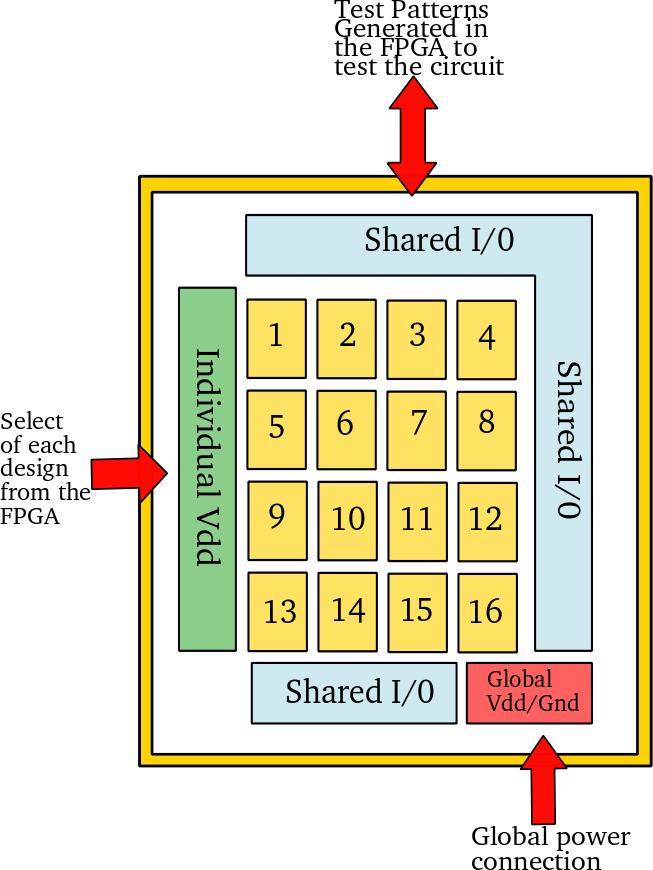
\includegraphics[scale=0.35]{Chip.png}
\caption{Overview of the Superchip (D2)}
\label{fig:chip_overview}
\end{figure}

All individual designs share the same 24 input and 24 output pins, but have separate power supplies.
As all of them share the same outputs, only one design can be active at any one time.
\\

Each of the 16 individual blocks on the chip is made up of smaller designs such as
adders, ring oscillators and other simple digital circuits. Every year one of the
smaller designs is an oscillator. As such, one of the requirements of the chip tester
is to measure the frequency of the on-chip oscillator.
\\

The chip tester was to be implemented using an Altera DE2-115 Development Board,
featuring an Altera Cyclone IV EP4CE115 FPGA.


\newpage
\section{DE2 Board Overview}
The DE2 board is an FPGA board designed by Terasic, based around an Altera
Cyclone IV FPGA. The following hardware relevant to this project is provided on
the DE2-115 board:

\begin{itemize}
 \item Altera Cyclone® IV EP4CE115 FPGA device
 \item USB Blaster (on board) for programming; both JTAG and Active Serial (AS) programming modes are supported
 \item 2MB SRAM (organized as 1M x 16 bits)
 \item 128MB SDRAM
 \item 8MB CFI Flash memory
 \item SD Card socket
 \item 50MHz oscillator
 \item 2 Gigabit Ethernet PHY with RJ45 connectors
 \item RS-232 transceiver and 9-pin connector
 \item One 40-pin Expansion Header with diode protection
 \item One High Speed Mezzanine Card (HSMC) connector
 \item 16x2 Character LCD display
\end{itemize}




\section{System Overview}
The Superchip tester designed within this project aims to provide a functional
and user friendly test environment for the University of Southampton Superchip.

The Superchip tester is able to test both the actual fabricated design and
a pre-fabrication version of it by using a secondary FPGA and programming it with
a hardware description of the design.

To achieve all of this, the chip tester consists of the following parts:

\begin{itemize}
 \item the main FPGA board (Altera DE2),
 \item the DUT board (Superchip),
 \item the secondary virtual design board (with programmable FPGA),
 \item the backend server (also providing a database and a web interface).
\end{itemize}

A graphical illustration of the overview of the system can be seen in figure \ref{fig:intro_sys_overview}.

\begin{figure}[h!]
\centering
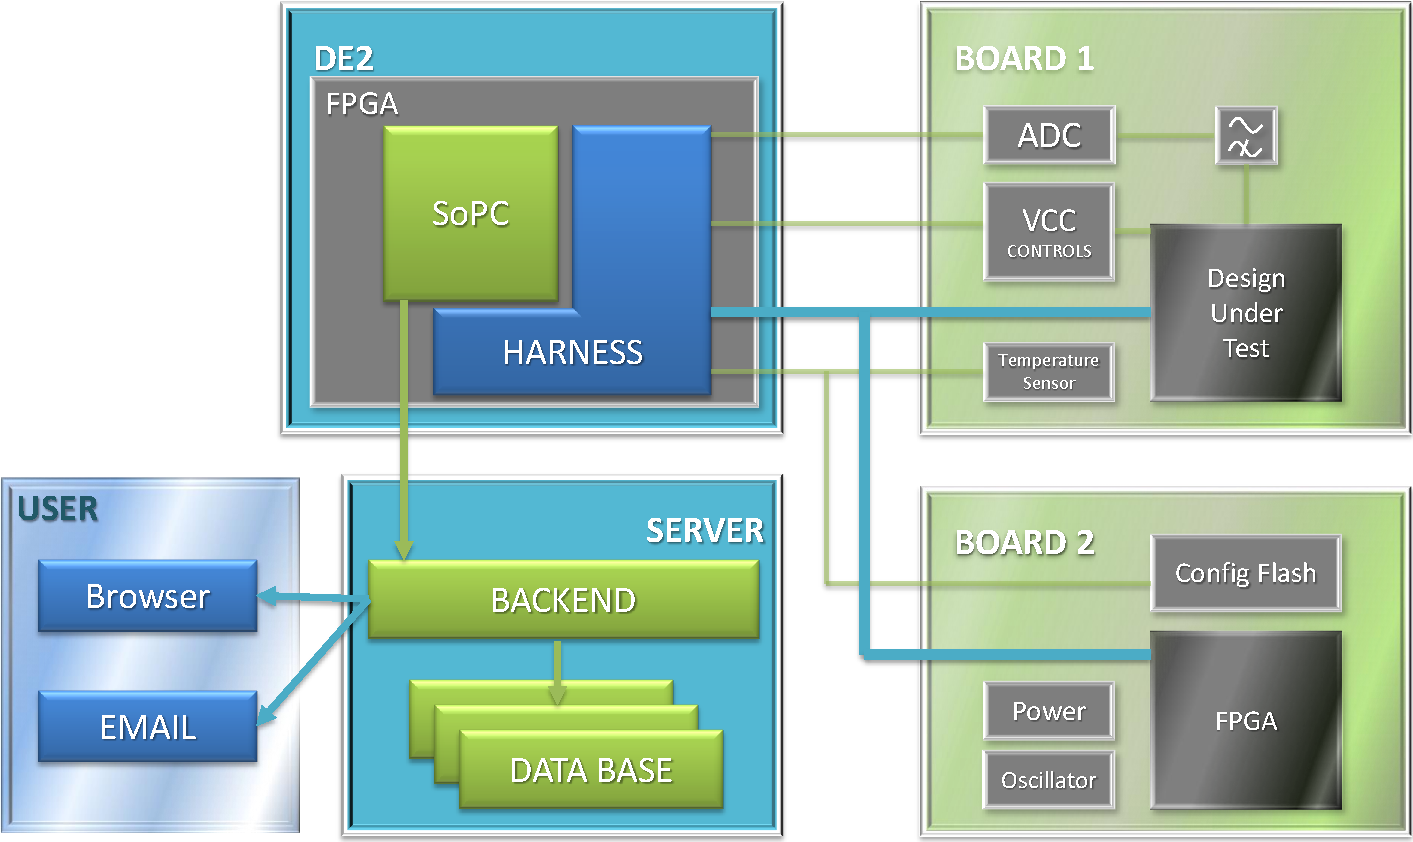
\includegraphics[width=0.9\textwidth]{sys_overview}
\caption{Overview of the ChipTester system designed for the ELEC6027 VLSI Group Design Project, Team I.}
\label{fig:intro_sys_overview}
\end{figure}


The DE2 main board hosts the System on Programmable chip (SoPC) core and the harness to
the device under test that provide the main functionality of
the designed system. The SoPC and harness implement
the chip testing functionality that is the main function of the project, implementing
vector testing for the digital part of the DUT as well as frequency measurement of
the oscillator on the DUT, ADC capture and slave FPGA reprogramming.

The two external boards can be connected via the HSMC connector to the DE2 main board.
Both boards share a similar pin-out for the device under test, so that both pre- and post-
fabrication designs can be tested in the same manner.

The primary DUT board provides a socket in which the final fabricated design can
be plugged in for testing. The board also includes an ADC and the Vcc control to be
able to switch individual designs on the superchip on and off.

The secondary board contains a slave FPGA and a configuration SPI flash and an oscillator for
use with the slave FPGA. This secondary FPGA can be programmed and controlled from the
main DE2 board without any hardware modifications, allowing for dynamic reconfiguration.
This allows the board to be used to test a pre-fabrication HDL description.
After reconfiguration of the slave FPGA the chip is tested in the same way as the real
design would be.

The main DE2 board communicates with a backend server via a simple HTTP API. The
backend server is able to store test results from the DE2 board in a database and
display them to the user via a user-friendly web interface. The web interface,
in addition to displaying results, also allows the users to upload a design and configuration
archive that is used to program slave FPGA with an arbitrary design and test it.

The backend is able to send out email summaries of test results as soon as they
come in from the main DE2 board.

An administration interface allowing for database management is also provided.










